\documentclass[11pt,a4paper]{article}

% --- Layout / style (keep your look) ---
\usepackage[margin=2.5cm]{geometry}
\usepackage{enumitem}
\usepackage{xcolor}
\usepackage{hyperref}
\usepackage{titlesec}
\usepackage{microtype}

% --- Figures ---
\usepackage{graphicx}
\usepackage{caption}
\usepackage{subcaption}

% Remove extra space after subsection (tight)
\titlespacing*{\subsection}{0pt}{1em}{-0.6em}
\titlespacing*{\section}{0pt}{1.2em}{0.2em}

% --- Link colors ---
\definecolor{LinkGreen}{RGB}{0,128,0}
\definecolor{LinkBlue}{RGB}{0,160,255}
\hypersetup{
  colorlinks=true,
  linkcolor=LinkGreen,
  urlcolor=LinkBlue,
  citecolor=LinkGreen
}

\setlength{\parindent}{0pt}
\setlength{\parskip}{0.6em}
\urlstyle{tt}

% Compact lists
\setlist[itemize]{leftmargin=1.5em, itemsep=0.2em, topsep=0.2em}
\setlist[enumerate]{leftmargin=1.5em, itemsep=0.2em, topsep=0.2em}

% Slightly tighter captions
\captionsetup{font=small, labelfont=bf}
\setlength{\abovecaptionskip}{4pt}
\setlength{\belowcaptionskip}{0pt}

\begin{document}

% =========================
% Title block
% =========================
\begin{center}
{\LARGE\bfseries Assignment 2 Report: Profiling Overestimation Bias in Ensemble Q-learning\par}
\vspace{0.5em}
{\normalsize DM 887 Reinforcement Learning - Spring 2026\par}
\vspace{0.8em}
\end{center}

\begin{center}
Jannik Busse Guldmand \\
\texttt{jagul24@student.sdu.dk} \\
Supervisor: Professor Melih Kandemir
\end{center}

\vspace{0.6em}

% =========================
% REPORT
% =========================
\section*{Rapport}

\subsection*{Goal}
The objective is to profile \emph{overestimation bias} by monitoring the gap between:
(i) the agent's \textbf{predicted} return from the start state and
(ii) the \textbf{observed} return of the current greedy policy, across training.
We compare four tabular ensemble Q-learning variants and study the effect of \textbf{algorithm choice}, \textbf{state size}, and \textbf{ensemble size}.

\subsection*{Environments (tabular, episodic, tunable state size)}
Three episodic environments were designed with a tunable number of states (target sizes: 10, 15, 20):
\begin{itemize}
  \item \textbf{Stochastic Corridor:} a narrow path from start to goal. Slip introduces stochastic transitions; reward noise introduces target variance.
  \item \textbf{Open Grid:} multiple paths to the goal; stochasticity makes the max-operator more prone to overestimation.
  \item \textbf{Hazard Grid:} same as open grid but with terminal holes (large negative reward), creating sharp value contrasts and risk-sensitive regions.
\end{itemize}
All environments use: step cost \(-1\), goal \(+100\), hole \(-100\), slip probability (stochastic transitions) and optional reward noise.

\subsection*{Algorithms (tabular Q ensembles)}
The following methods were implemented and compared:
\begin{itemize}
  \item \textbf{Double Q-learning (Double Q)}: decouples action selection and evaluation using two tables (van Hasselt, 2010).
  \item \textbf{DQN-min}: min-clipped target using two critics, as in TD3-style clipped double Q (Fujimoto et al., 2018).
  \item \textbf{Q-ensemble-min}: min-clipping across all ensemble members (N$>$2).
  \item \textbf{REDQ}: min-clipping across a randomly sampled subset (pair) from an ensemble (Chen et al., 2021).
\end{itemize}

\subsection*{Experimental setup and bias metric}
Training uses tabular Q-learning with \(\gamma=0.99\), \(\alpha=0.1\), and \(\epsilon\)-greedy exploration with linear decay (1.0 \(\rightarrow\) 0.05) over 500 episodes.
For each configuration we run multiple seeds and report mean behavior.

At evaluation checkpoints, we compute:
\begin{itemize}
  \item \textbf{Predicted value:} \(\hat{V}(s_0)=\max_a \overline{Q}(s_0,a)\), where \(\overline{Q}\) is the mean across the ensemble.
  \item \textbf{Observed value:} average discounted return from executing the \emph{greedy policy} (no exploration) for multiple rollouts.
  \item \textbf{Overestimation bias:} \(b=\hat{V}(s_0)-V^{\pi_{\text{greedy}}}(s_0)\).
\end{itemize}

\subsection*{Results}
Figure~\ref{fig:biasmag} summarizes the bias magnitude across all three environments and state sizes (N=5 for ensemble methods). Figure~\ref{fig:learning} shows learning curves.

\begin{figure}[t]
  \centering
  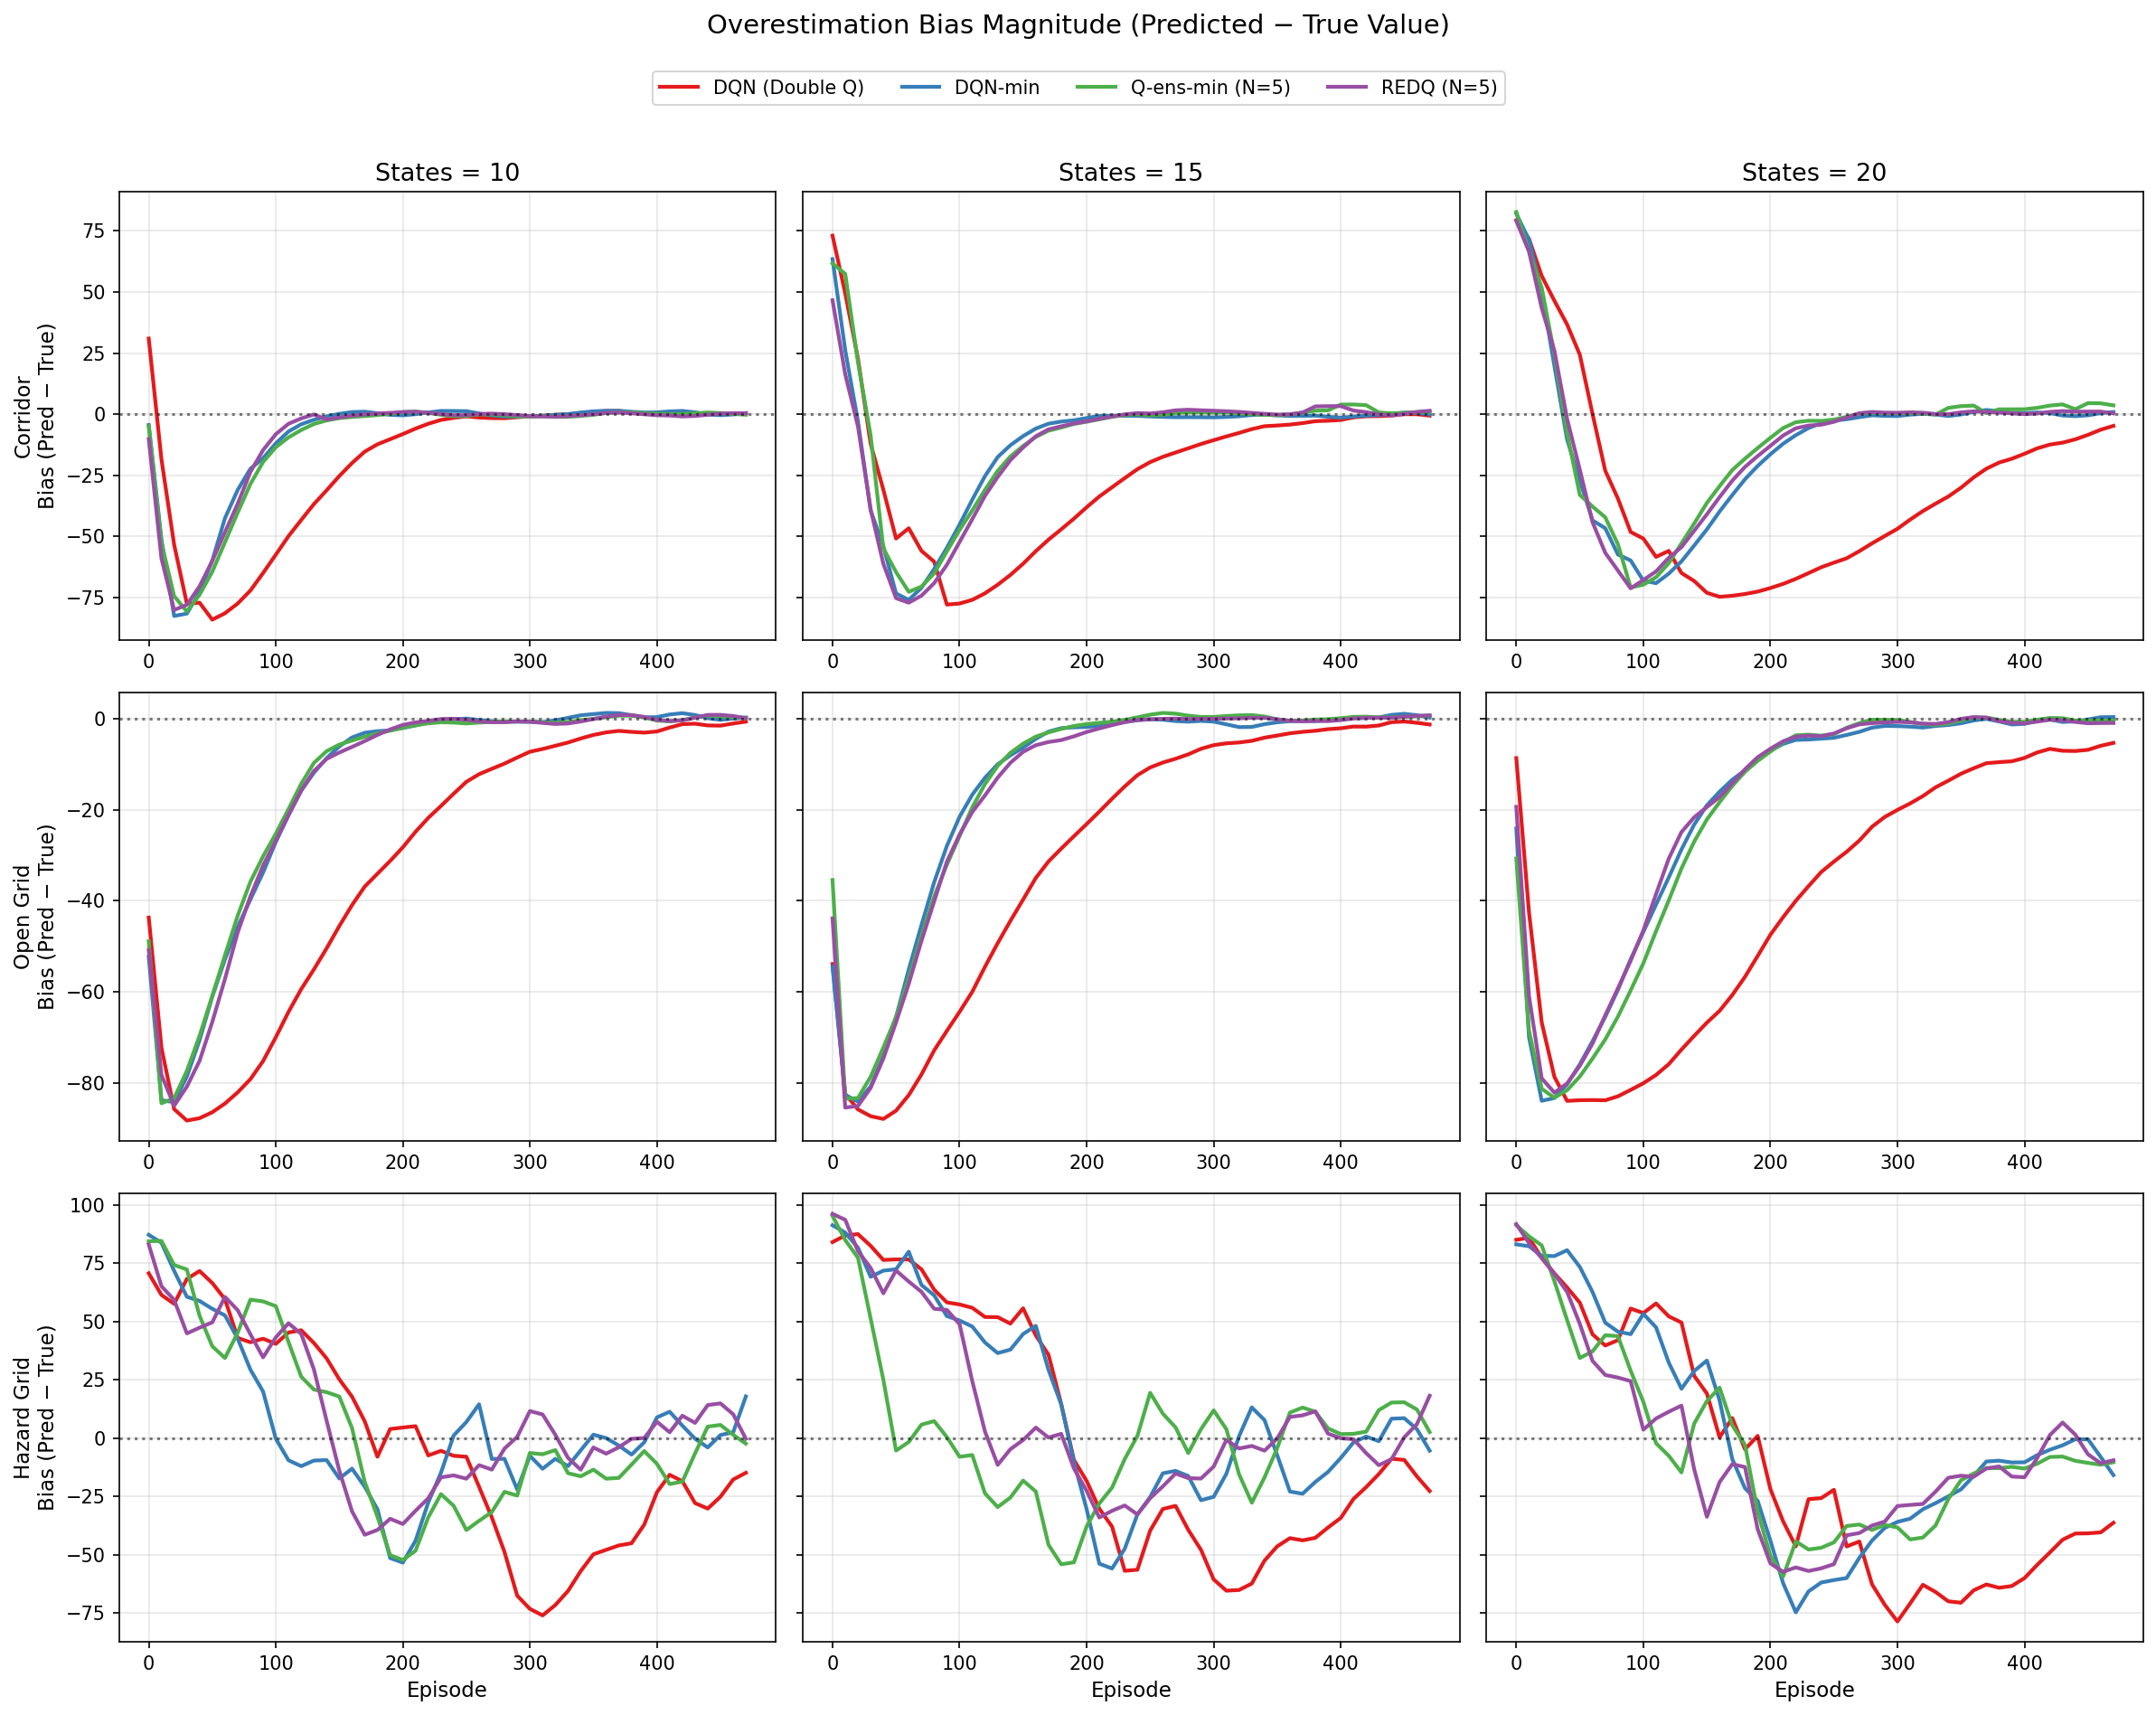
\includegraphics[width=0.98\linewidth]{overestimation_magnitude.png}
  \caption{Overestimation bias magnitude (Predicted -- Observed) across environments and state sizes.}
  \label{fig:biasmag}
\end{figure}

\begin{figure}[t]
  \centering
  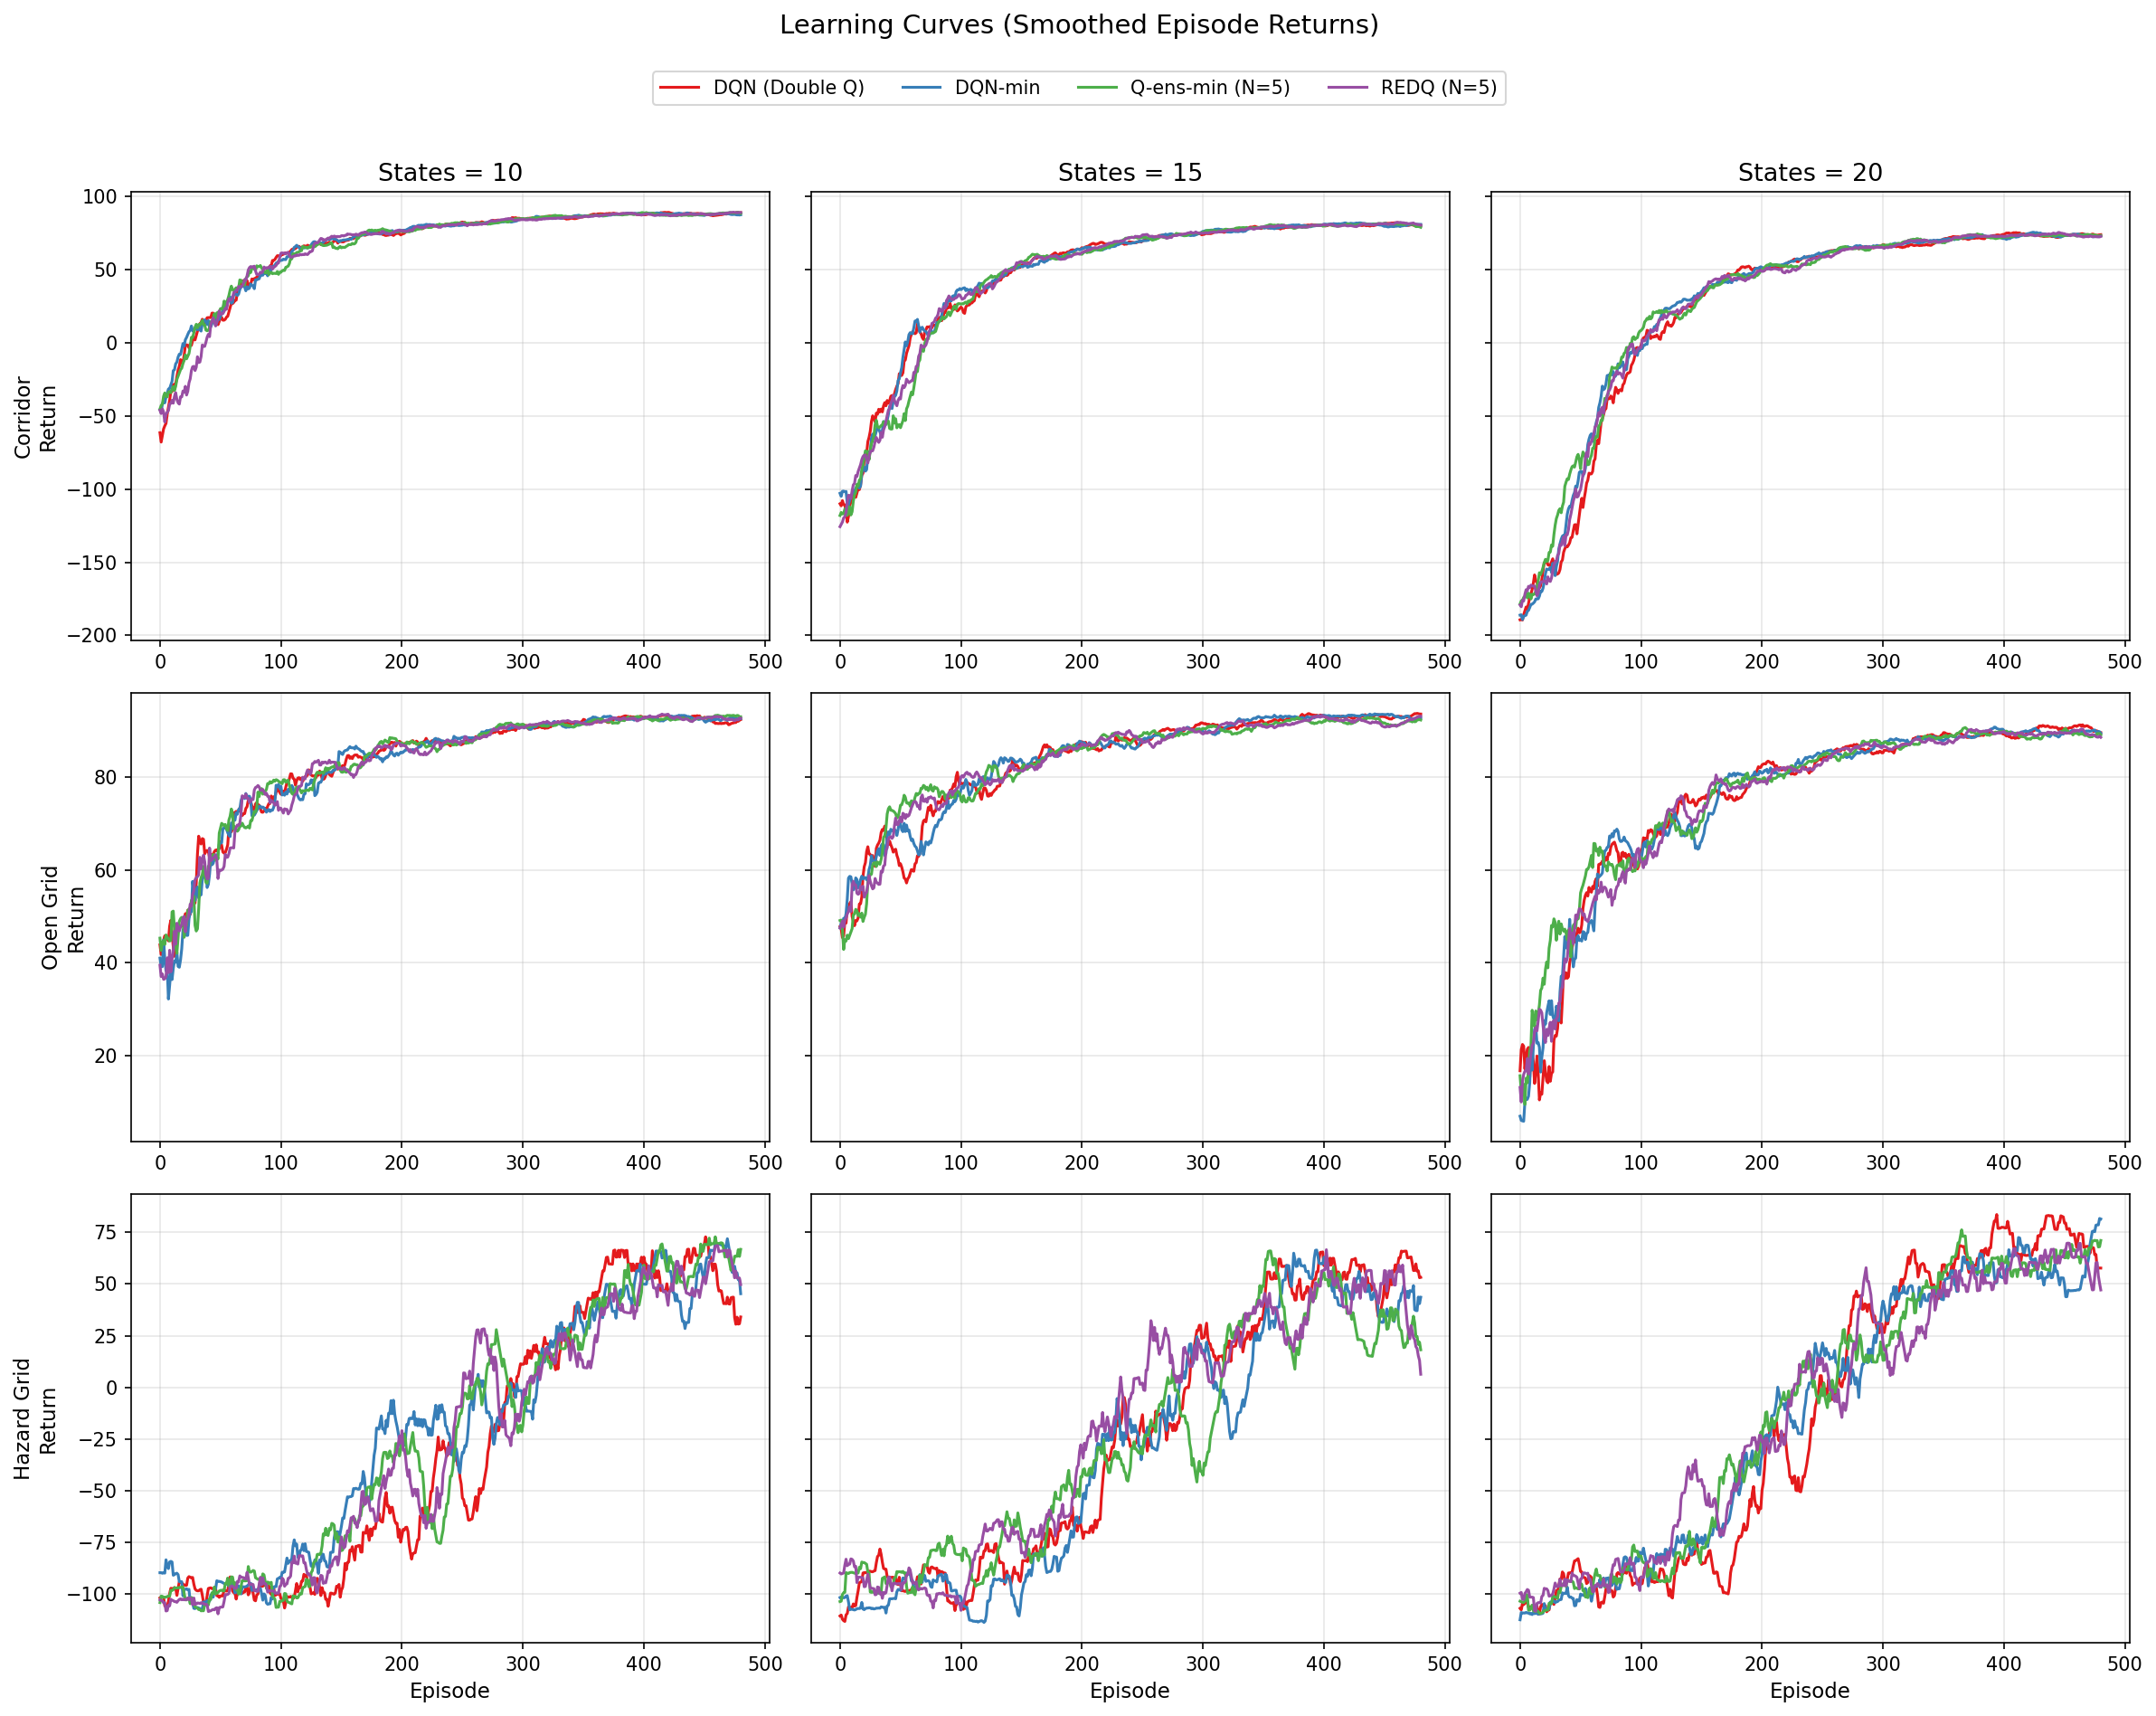
\includegraphics[width=0.98\linewidth]{learning_curves.png}
  \caption{Learning curves (smoothed episode returns) across environments and state sizes.}
  \label{fig:learning}
\end{figure}

\subsection*{Discussion (bias vs learning)}
Across environments, methods that apply \textbf{min-clipping} reduce positive overestimation bias compared to standard Double Q-learning. Stronger min-clipping (full ensemble min) tends to be more conservative, which can reduce bias but may also slow early learning depending on the environment’s stochasticity and the prevalence of sharp negative terminal outcomes (hazards).

The relationship between bias and learning curves is consistent with the RL interpretation: overestimation inflates targets, which can speed up apparent value growth but may destabilize learning and lead to suboptimal policies in risky regions (especially in the hazard environment). Min-clipping reduces target inflation and typically yields smoother, more reliable improvement.

\subsection*{Ensemble size effect}
Figure~\ref{fig:ens} isolates the effect of ensemble size (state size fixed to 15). Increasing ensemble size changes the strength/variance of the min-reduction: full min-clipping typically becomes more conservative with larger N, while REDQ’s randomized pairwise min provides a compromise between bias reduction and optimism.

\begin{figure}[t]
  \centering
  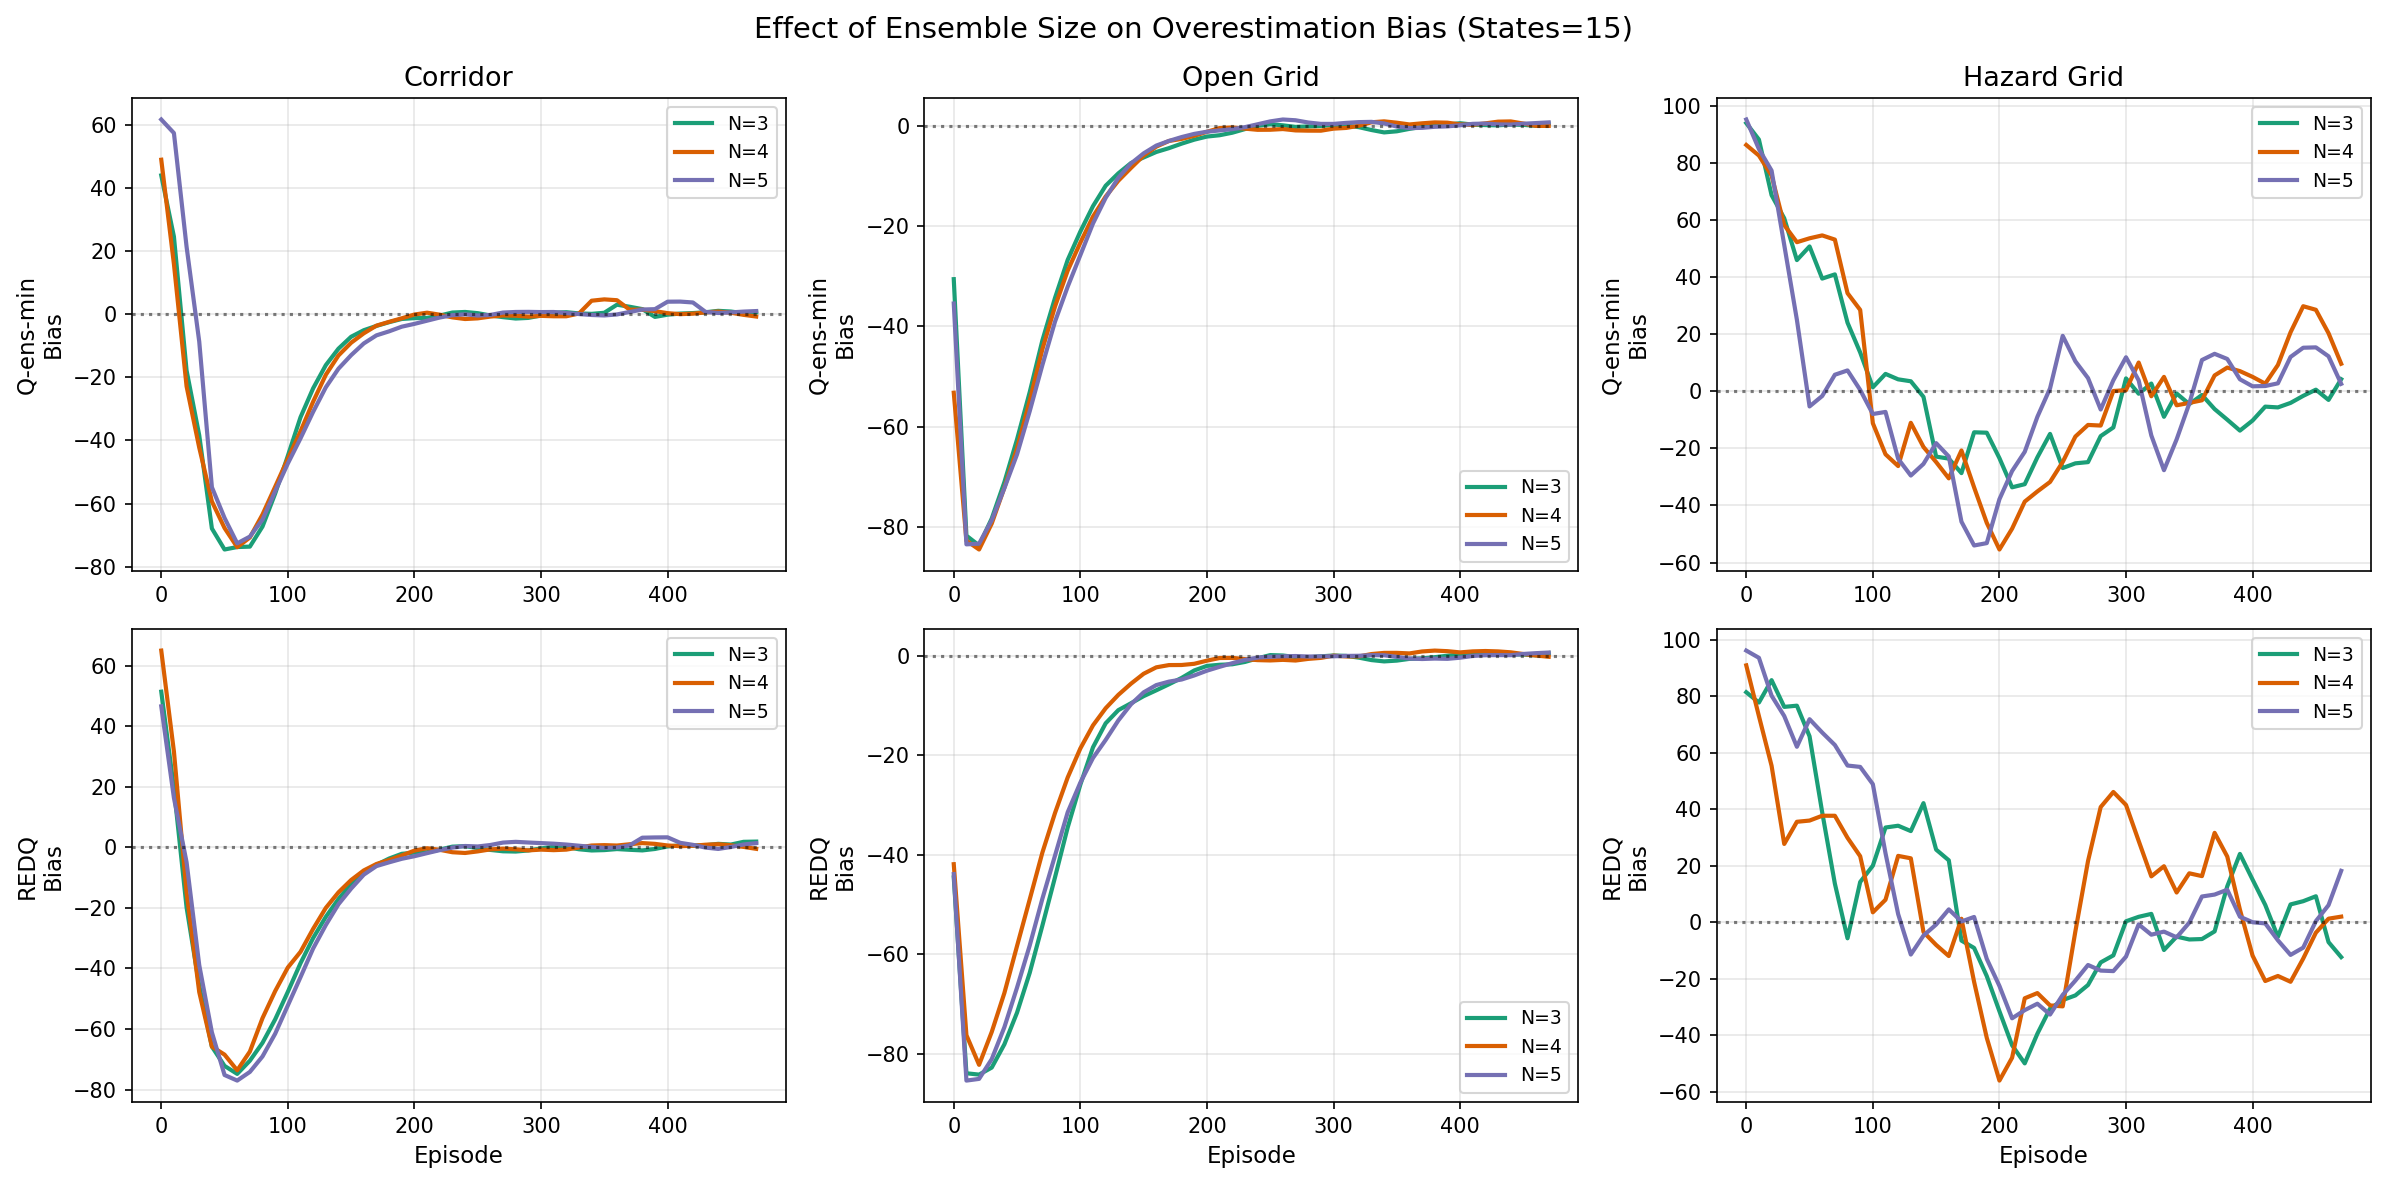
\includegraphics[width=0.98\linewidth]{ensemble_size_effect.png}
  \caption{Effect of ensemble size on overestimation bias (states=15).}
  \label{fig:ens}
\end{figure}

\vspace{0.2em}

\subsection*{AI Usage (Disclaimer)}
Claude Opus 4.6 was used to support the development of (1) the experimental design and
(2) the implementation for Assignment \#2, using GridWorld and ObjectRL.
Notion AI was used to support drafting and editing the report text in \LaTeX{}.

% =========================
% APPENDIX / BILAG
% =========================
\clearpage
\section*{Appendix (Bilag): Additional Plots}

\begin{figure}[h]
  \centering
  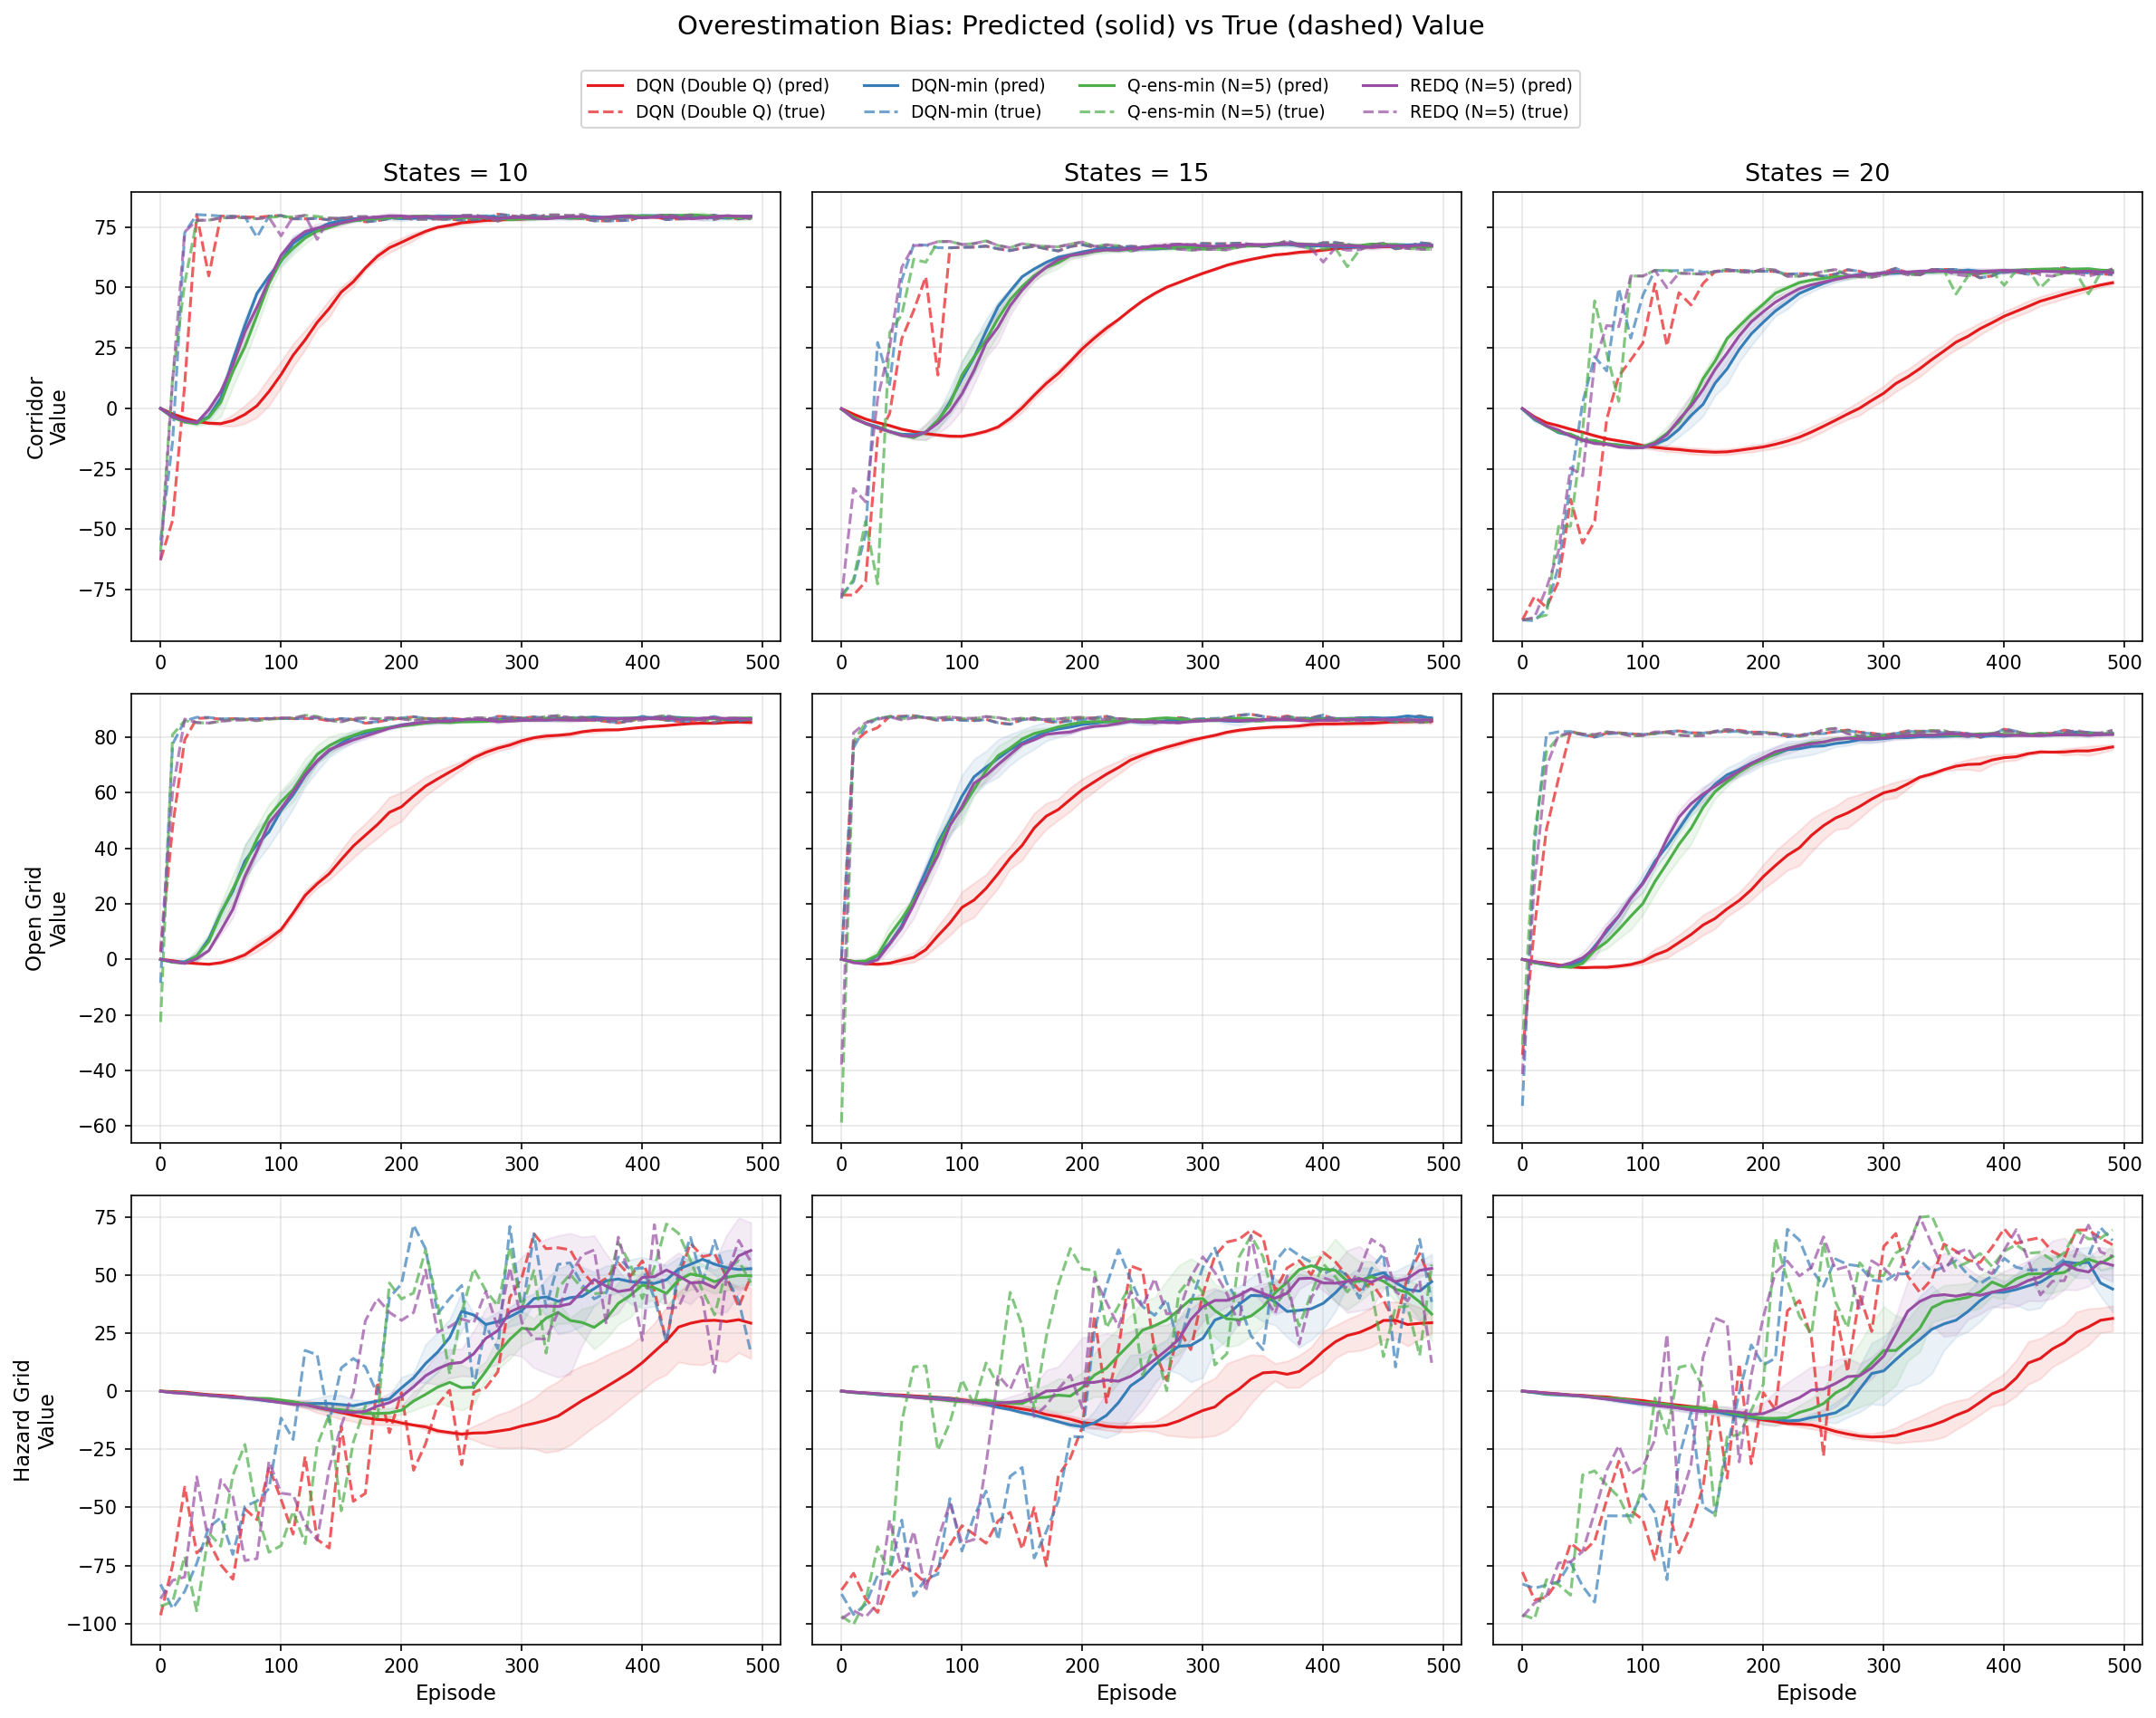
\includegraphics[width=0.98\linewidth]{overestimation_bias.png}
  \caption{Predicted (solid) vs observed (dashed) value during training.}
\end{figure}

\begin{figure}[h]
  \centering
  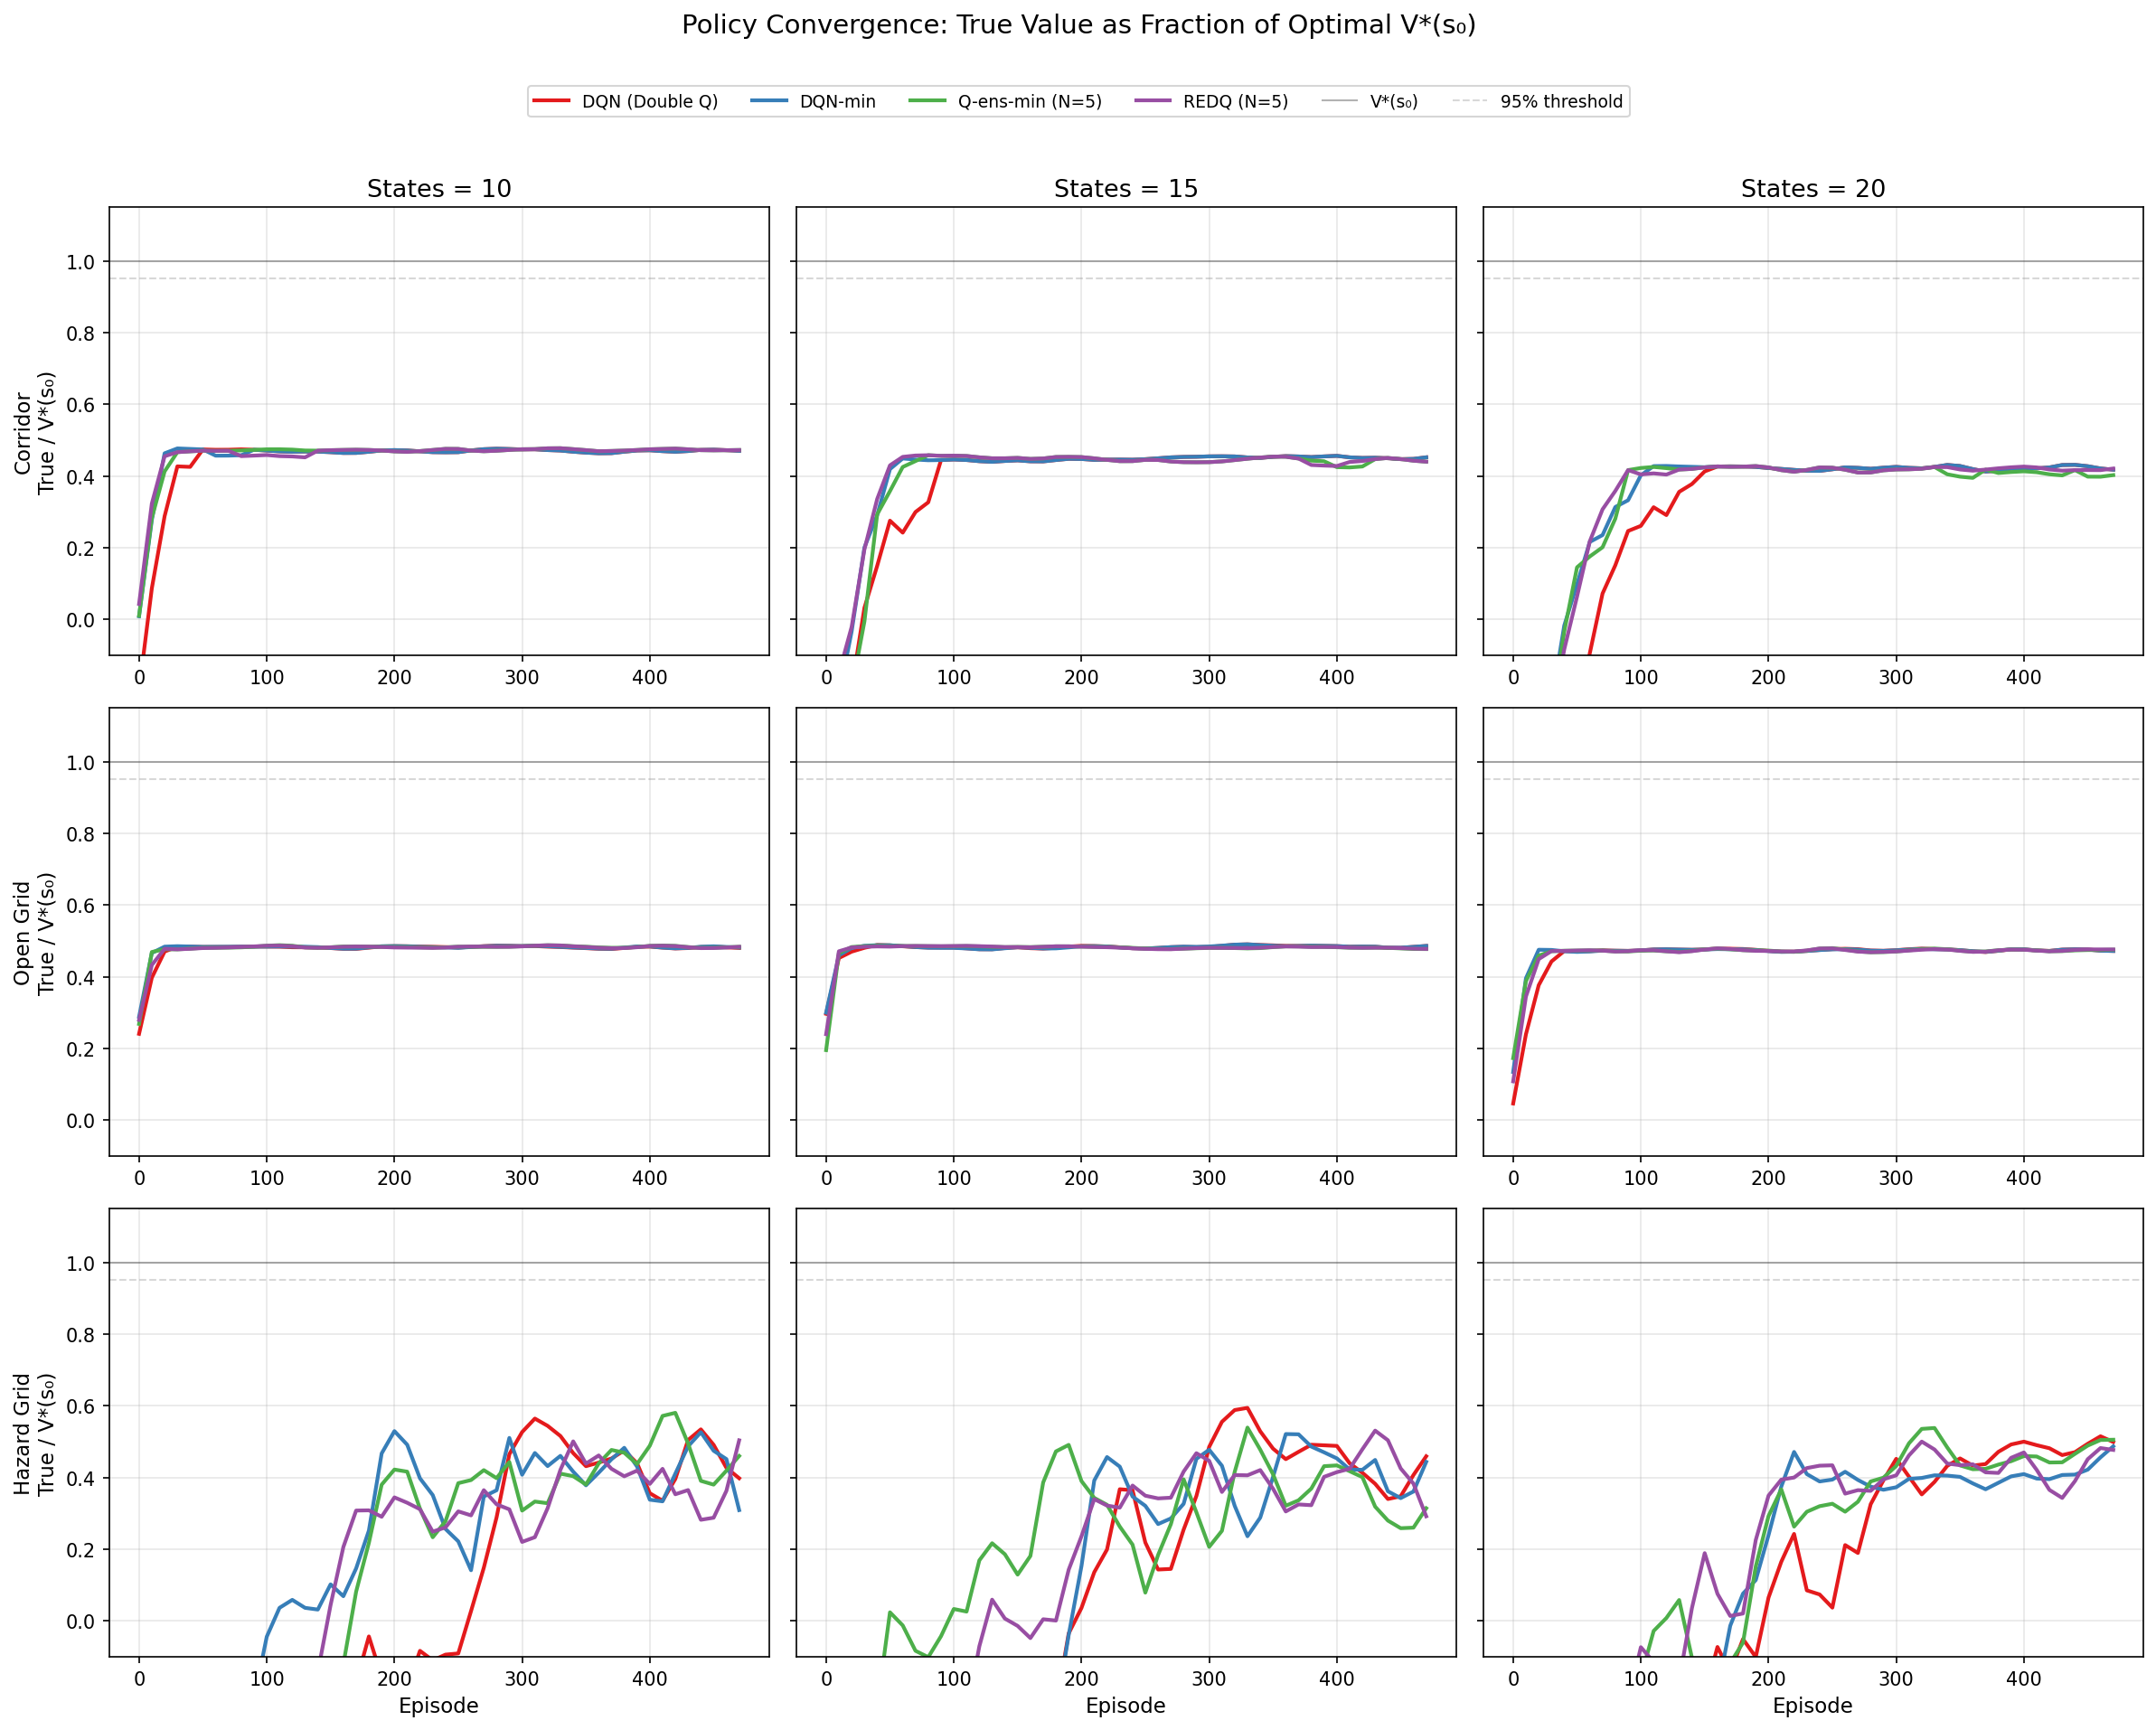
\includegraphics[width=0.98\linewidth]{policy_convergence.png}
  \caption{Policy convergence (true value as fraction of optimal \(V^*(s_0)\)).}
\end{figure}

% =========================
% REFERENCES (only if used)
% =========================
\clearpage
\section*{References}

\begin{enumerate}[label={[}\arabic*{]}, leftmargin=1.8em]
  \item \label{hasselt2010}
  H. van Hasselt.
  \textit{Double Q-learning}.
  NeurIPS, 2010.

  \item \label{fujimoto2018}
  S. Fujimoto, H. van Hoof, D. Meger.
  \textit{Addressing Function Approximation Error in Actor-Critic Methods} (TD3).
  ICML, 2018.

  \item \label{chen2021}
  X. Chen, Z. Wang, E. Zhou, et al.
  \textit{Randomized Ensembled Double Q-Learning: Learning Fast Without a Model}.
  ICLR, 2021.
\end{enumerate}

\end{document}